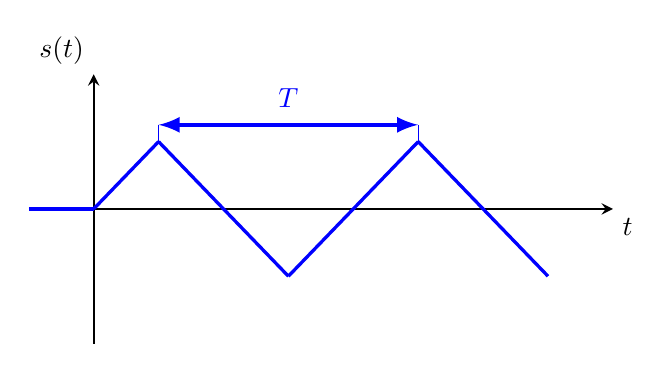
\begin{tikzpicture}
    \begin{axis}
    [	ticks=none,
        axis line style = thick,
        height=5cm,
        width=9cm,
        axis x line=center,
        axis y line=center,
        xmin=-2,
        xmax=16,
        ymin=-2.0,
        ymax=2.0,
        xlabel={$t$},
        ylabel={$s(t)$},
        xlabel style={below right},
        ylabel style={above left},
        clip bounding box=upper bound,
        enlargelimits=false
    ]
    \addplot[very thick,blue,domain=-2:0, samples=101] {0};
    \addplot[very thick,blue,domain=0:2, samples=101]  {0.5*x};
    \addplot[very thick,blue,domain=2:6, samples=101]  {-0.5*x+2};
    \addplot[very thick,blue,domain=6:10, samples=101] {0.5*x-4};
    \addplot[very thick,blue,domain=10:14, samples=101]{-0.5*x+6};
    \draw[blue] (axis cs:2,1) -- (axis cs:2,1.25);
    \draw[blue] (axis cs:10,1) -- (axis cs:10,1.25);
    \draw[blue,ultra thick, latex-latex] (axis cs:2,1.25) -- 
    node[above,yshift=+0.2em]{$T$} (axis cs:10,1.25);
    \end{axis}
\end{tikzpicture}
